%!TEX root = ../main.tex

\chapter{Solution of Dynamic Systems Described by Differential-Algebraic Equations}
\label{chap4:daes}

In this chapter, we present an algorithm for the index reduction of first-order \acp{DAE}. The proposed approach can be applied to generic \acp{DAE} and exploits neither a priori knowledge nor ad hoc techniques to leverage the specific formulation of the system. The index reduction is performed only by using symbolic manipulation and linear algebra techniques. It is based on the successive separation of the differential and algebraic equations of the system and the subsequent differentiation of the algebraic part. Improved symbolic matrix factorization is used to perform the \acp{DAE} partitioning, ensure numerical stability, and limit the expression swell of the reduced-index system. The effectiveness of the algorithm will be validated in the next chapter through a set of examples on a wide range of systems, including physical systems, engineering applications, and ``artificial'' \acp{DAE} with specific properties. The proposed symbolic index reduction algorithm is implemented in \Maple{} as part of an open-source library.

% % % % % % % % % % % % % % % % % % % % % % % % % % % % % % % % % % % % % % % %

\section{Differential-Algebraic Equations Index Reduction and Solution}
\label{chap4:sec:introduction}

As we already mentioned in Chapter~\ref{chap2:brief_daes}, \acp{DAE} are extensively used in dynamic system modeling. The challenge in numerically solving a \ac{DAE} system is assessed through its differentiation index, commonly referred to as ``the'' index~\cite{campbell1995index, campbell1995highindex}. Achieving accurate simulations necessitates converting high-index \acp{DAE} into low-index counterparts, posing a well-recognized challenge~\cite{petzold1982differential}. This process involves transforming a \ac{DAE} system into an equivalent system with a lower index through successive differentiation of the system equations. For this reason, the differentiation index is roughly defined as the number of times algebraic equations are differentiated to obtain an equivalent system of \acp{ODE} with invariants. Index reduction is a crucial step prior to the numerical integration of \acp{DAE}, as integrating high-index systems can be impractical. The primary obstacle lies in the necessity to solve non-linear systems of equations at each integration step, which can be computationally expensive and, in certain cases, numerically unstable. Specific numerical techniques, introduced in~\cite{petzold1982differential, thomsen1999numerical, baumgarte1972stabilization}, have been developed to address this challenge. However, these methods are not universally effective and may be inapplicable to some high-index \acp{DAE}. Consequently, index reduction becomes an indispensable preliminary stage before numerical integration~\cite{lamour2013differential}.

Given its complicated nature, index reduction has been the subject of extensive research and is often carried out by leveraging the specific formulation of the \ac{DAE} system, like in the multi-body modeling~\cite{zhou2005implicit, zhou2007symbolic, zhou2007symbolicseq, bayo1988modified, wehage1982generalized}. When the specific formulation of the \ac{DAE} system is not known a priori, or the system is not in a specific form, the index reduction process becomes more challenging. Many current simulation software packages for dynamic systems use index-reduction algorithms based on the \ac{SA} of the system, such as the Pantelides algorithm~\cite{pantelides1988consistent} and the dummy derivatives method~\cite{mattsson1993index}, which are subcases of the Pryce's $\Sigma$-method~\cite{pryce1998solving, pryce2001simple, nedialkov2007solvingI, nedialkov2007solvingII, nedialkov2008solvingIII, nedialkov2015algorithm, tan2016symbolic, mckenzie2017structural}. These algorithms are effective in reducing the index of most of the systems, but they can fail either for numerical cancellations~\cite{iwata2019index} or underestimation of the differentiation index~\cite{pantelides1988consistent, unger1995structural}, like in the case of Rei{\ss}ig's \acp{DAE} family~\cite{reissig2000differential}. Symbolic manipulation is proven to be successful in restating a \acp{DAE} on which the $\Sigma$-method fails to a \acp{DAE} on which the \ac{SA} may succeed~\cite{tan2016symbolic}.

Index reduction based on symbolic-numeric aided \ac{SA} has been successful in handling failures of the Pryce's $\Sigma$-method~\cite{tan2016symbolic} as well as in performing symbolically-informed \ac{SA}~\cite{chowdhry2004symbolic}. This latter \ac{SA} approach, which is named $\sigma v$-method, uses symbolic-numeric \ac{LU} factorization for variable substitution and rank determination on linear constant coefficient \acp{DAE}. A valuable attempt to use pure symbolic manipulation in \acp{DAE} index reduction is presented in~\cite{zhou2005implicit, zhou2007symbolic, zhou2007symbolicseq}, where implicit involutive form and \ac{LU} decomposition are successfully used to reduce the index of a simple constrained multi-body system. It is clear that index reduction algorithms based on pure symbolic matrix factorization represent a viable alternative to classic \ac{SA} techniques. However, symbolic matrix factorization feasibility is strongly tied to the performance of the symbolic computation kernel and its capabilities~\cite{zhou2008fraction}. Large expressions can lead to strong performance degradation of the kernel. Techniques aimed at limiting this decrease of performance while performing symbolic linear algebra operations are presented in~\cite{zhou2006hierarchical, zhou2007symbolic, zhou2007symbolicseq}. In these works, the hierarchical representation of expressions is applied to matrix factorization tasks. Nonetheless, the \LULEM{} package~\cite{carette2006linear}, which implements large expression management strategies in \ac{LU} decomposition, significantly outperforms the \Maple{}'s built-in matrix factorization routines.

The absence of user-invocable standalone functions within the \Maple{} environment that allows for the automatic index reduction of \acp{DAE}, and the inability to extract both the reduced-index system and invariants from the \texttt{dsolve} function, are the primary motivations of this research. Furthermore, recent advances in symbolic matrix factorization, combined with expressions hierarchical representation techniques, provide valuable tools that enable us to further investigate the applicability of a novel algorithm for the index reduction of \ac{DAE} systems, firstly presented in~\cite{stocco2024symbolic} as a preliminary work. The proposed methodology is similar to the previous work of~\citet{chowdhry2004symbolic} and extends it to generic first-order \acp{DAE}, linear in the states' derivatives. Nonetheless, the proposed algorithm does not work on the structural matrix of the system but on the \ac{DAE} system symbolic expressions. Specifically, the idea of using matrix factorization for variable substitution and rank determination is adopted to iteratively separate the differential and algebraic equations of the system. The algebraic equations are then differentiated to obtain an equivalent system with a lower differentiation index. Not less important, new libraries for symbolic matrix factorization (\LAST{}), large expression management (\LEM{}), and signature computation (\SIG{}) are presented. These libraries are based on the \LULEM{} package and extend the work of~\citet{zhou2006hierarchical, carette2006linear} and~\citet{zhou2007symbolic}. The newly presented libraries are designed to ensure the numerical stability of the numerically evaluated expressions, limit the expression swell, and provide an updated object-oriented interface. The effectiveness of the presented index reduction algorithm is validated through symbolic-numerical examples on a wide range of systems, including physical systems, engineering applications, as well as ``artificial'' systems with specific properties. The proposed algorithm is implemented in the \Maple{} environment and is available as a collection of open-source packages~\cite{last, lem}. Furthermore, the insights and the techniques presented in~\cite{zhou2006hierarchical, carette2006linear, zhou2007symbolic} are used to improve the presented algorithm to embed the hierarchical representation of expressions in a future implementation of the algorithm.

%This chapter is organized as follows. After this introduction (Section~\ref{chap4:sec:introduction}), the index reduction algorithm is presented in Section~\ref{chap4:sec:algorithm}. The expression swell mitigation, as well as the details on the symbolic matrix factorization, are discussed in Sections~\ref{chap4:sec:expression_swell} and \ref{chap4:sec:matrix_factorization}. The effectiveness of the algorithm is showcased through symbolic-numerical examples in Section~\ref{chap4:sec:example}. Finally, Sections~\ref{chap4:sec:future_work} and~\ref{chap4:sec:conclusions} report future developments and conclusions respectively. In~\ref{chap4:sec:cokernel} details on cokernel computation are reported. The newly developed object-oriented symbolic linear algebra (\ref{chap3:sec:last}), large expression management (\ref{chap3:sec:lem}) and signature computation (\ref{chap4:sec:signature}) package descriptions are also included in the appendices. The symbolic index reduction algorithm is implemented in the \Maple{} language and is available as part of the open-source \Indigo{} library~\cite{indigo}. Its usage is illustrated in~\ref{chap4:sec:index_reduction}.

% % % % % % % % % % % % % % % % % % % % % % % % % % % % % % % % % % % % % % % %

\section{A New Index Reduction Algorithm}
\label{chap4:sec:algorithm}

In this section, we explore the theoretical aspect of reducing the differential index of \ac{DAE} systems. Specifically, to systematically reduce the \ac{DAE} system's index, a novel iterative algorithm is presented. This algorithm comprises two main phases: initially, the separation of the differential equations from the algebraic equations inherent in \acp{DAE}; and subsequently, the differentiation of the algebraic ones to obtain an equivalent system with a reduced index. The algorithm that is presented in this section is implemented in the \Maple{} environment and is available as an open-source package~\cite{indigo}.

\subsection{Differential and Algebraic Equations Separation}
\label{chap4:sec:separation}

The initial phase of the index reduction procedure involves the partitioning of the \ac{DAE} system into its differential and algebraic equations. While in the case of small systems this can be accomplished through manual identification and isolation of the algebraic equations, this approach is inconvenient when dealing with large systems. An alternative method for automating the separation process leverages the cokernel, or left null space, of the \ac{DAE} system matrix, which is computed through matrix factorization techniques. The usage of the cokernel offers a more efficient and reliable means of accomplishing the separation task, variable substitution and not less importantly rank determination.

Consider a first-order system of \acp{DAE} $\mF$ of the form
%
\begin{equation}
  \label{chap4:eq:daes}
  \mF = \mA \, \mxp - \mb = \m{0}  \, \text{.}
\end{equation}
%
We denote the cokernel and its orthogonal complement of $\mA$ with $\mK$ and $\mN$ respectively (see~\ref{chap4:sec:cokernel} for details on the cokernel computation with symbolic matrix factorization). Notice that the cokernel is the subspace obtained by the span of $\mK$'s columns. For this reason, hereafter, we refer to the cokernel as the matrix $\mK$ whose columns span the cokernel. Using $\mK$ and $\mN$ it is possible to separate the algebraic part of the \acp{DAE}~\eqref{chap4:eq:daes} as
%
\begin{equation}
  \label{chap4:eq:separated_daes}
  \begin{cases}
    \mE \, \mxp = \mg \\[0.1em]
    \ma = \m{0}
  \end{cases} \text{,} \quad \text{where} \qquad \mA = \begin{bmatrix}
    \mE \\[0.2em]
    \m{0}
  \end{bmatrix} \text{,}
  \quad \text{and} \quad
  \mb = \begin{bmatrix}
     \mg \\[0.2em]
     \ma
  \end{bmatrix} \, \text{.}
\end{equation}
%
The separated equations of the \acp{DAE} are obtained by the left product of $\mK$ and $\mN$ as
%
\begin{equation*}
  \begin{array}{l@{~}c@{~}l}
    \mE &=& \mN \, \mA \, \text{,} \\[0.1em]
    \mg &=& \mN \, \mb \, \text{,} \\[0.1em]
    \ma &=& \mK \, \mb \, \text{.}
  \end{array}
\end{equation*}
%
This results in an equivalent \ac{DAE} system, where the algebraic equations $\ma$ are now explicit. The details of the cokernel and its orthogonal complement computation are discussed in~\ref{chap4:sec:cokernel}.


\subsubsection{Cokernel Computation with Matrix Factorization}
\label{chap4:sec:cokernel}

The cokernel of a generic matrix $\m{A}$ is denoted as $\m{K}$ and satisfy $\m{K}\m{A} = \m{0}$. As mentioned before, the cokernel is the subspace obtained by the span of $\m{K}$'s columns. The orthogonal complement of the cokernel is denoted as $\m{N}$, moreover, the matrices $\m{N}$ and $\m{K}$ stacked compose a square non-singular matrix. It is common knowledge that matrix factorization techniques can be employed to compute the cokernel and its orthogonal complement. Among these techniques, the \ac{LU} factorization stands out as one of the most frequently used methods.

\paragraph{Lower-Upper Decomposition}

The full-pivoting \ac{LU} decomposition of a matrix $\m{A} \in \mathbb{R}^{m \times n}$ (with $m\geq n$) is represented as the product of matrices $\m{L}$ and $\m{U}$ with the permutation matrices $\mP$ and $\mQ$. It is characterized by the following properties:
%
\begin{itemize}
  \setlength{\itemsep}{0.0em}
  \item $\mP\m{A}\mQ = \m{L}\m{U}$;
  \item $\m{L} \in \mathbb{R}^{m \times m}$ is a lower-triangular matrix with all diagonal entries equal to $1$;
  \item $\m{U} \in \mathbb{R}^{m \times n}$ is an upper-triangular matrix;
  \item $\mP \in \mathbb{R}^{m \times m}$ and $\mQ \in \mathbb{R}^{n \times n}$ are the rows and columns permutation matrices, respectively.
\end{itemize}
%
If $\m{M}$ is defined such that $\m{M} = \m{L}^{-1}\mP$, then the following relation holds
%
\begin{equation*}
    \m{M}\m{A}
    = \m{L}^{-1}\mP\m{A}
    = \m{L}^{-1}\mP\m{A}\mQ\mQ^\top
    = \m{L}^{-1}\m{L}\m{U}\mQ^\top
    = \m{U}\mQ^\top
    = \begin{bmatrix} \m{U}_1 \\[0.2em] \m{0} \end{bmatrix}\mQ^\top \text{.}
\end{equation*}
%
If the identity matrix $\mI$ is partitioned as
%
\begin{equation*}
  \mI = \begin{bmatrix}
    \mI_1 & \m{0} \\[0.2em]
    \m{0} & \mI_2
  \end{bmatrix} \text{,}
  %
  \quad \text{where} \quad
  %
  \begin{array}{l}
    \mI_1 \in \mathbb{R}^{m \times m} \quad \text{and} \quad
    \mI_2 \in \mathbb{R}^{(m-n)\times(m-n)}\text{,}
  \end{array}
\end{equation*}
%
we can write
%
\begin{equation*}
  \begin{bmatrix} \mI_1 & \m{0} \end{bmatrix} \, \m{M}\m{A} =
  \begin{bmatrix} \mI_1 & \m{0} \end{bmatrix}
  \begin{bmatrix} \m{U}_1 \\[0.2em] \m{0} \end{bmatrix} \mQ^\top = \m{U}_1 \mQ^\top \text{,}
  %
  \qquad \text{and} \qquad
  %
  \begin{bmatrix} \m{0} & \mI_2 \end{bmatrix} \, \m{M}\m{A} =
  \begin{bmatrix} \m{0} & \mI_2 \end{bmatrix}
  \begin{bmatrix} \m{U}_2 \\[0.2em] \m{0} \end{bmatrix} \mQ^\top = \m{0} \text{.}
\end{equation*}
%
Eventually, the matrices $\m{N}$ and $\m{K}$ have the following form
%
\begin{equation*}
  \m{N} = \begin{bmatrix} \mI_1 & \m{0} \end{bmatrix} \, \m{M}
  %
  \quad \text{and} \quad
  %
  \m{K} = \begin{bmatrix} \m{0} & \mI_2 \end{bmatrix} \, \m{M},
\end{equation*}
%
where
%
\begin{equation*}
  \begin{array}{l}
      \m{K}\m{A} = \m{0} \\[0.2em]
      \m{N}\m{A} = \m{U}_1 ~ \text{is full-rank}
  \end{array} \, \text{,}
  %
  \quad \text{and} \quad
  %
  \begin{bmatrix} \m{N} \\[0.2em] \m{K} \end{bmatrix} \quad \text{is non-singular.}
\end{equation*}

\paragraph{Fraction-Free Lower-Upper Decomposition}

The \ac{FFLU} factorization is a variant of the \ac{LU} decomposition. It is based on the same principles as the standard \ac{LU} decomposition, but it is designed to avoid the appearance of fractions in the intermediate results. Similarly to the \ac{LU} case, the \ac{FFLU} decomposition of a matrix $\m{A} \in \mathbb{R}^{m \times n}$ (with $m\geq n$) is represented as the quintet of matrices $\m{L}$, $\m{U}$, $\m{D}$, $\mP$, and $\mQ$, and is characterized by the properties:
%
\begin{itemize}
  \setlength{\itemsep}{0.0em}
  \item $\mP\m{D}\m{A}\mQ = \m{L}\m{U}$;
  \item $\m{L} \in \mathbb{R}^{m \times m}$ is a lower-triangular matrix with all diagonal entries equal to $1$;
  \item $\m{D} \in \mathbb{R}^{m \times m}$ is a diagonal matrix;
  \item $\m{U} \in \mathbb{R}^{m \times n}$ is an upper-triangular matrix;
  \item $\mP \in \mathbb{R}^{m \times m}$ and $\mQ \in \mathbb{R}^{n \times n}$ are the rows and columns permutation matrices, respectively.
\end{itemize}
%
The procedure for computing the cokernel of a matrix $\m{A}$ using the \ac{FFLU} is similar to the case of the \ac{LU} decomposition. The only difference is in the computation of the matrix product $\m{M}\m{A}$. If $\m{M} = \m{L}^{-1}\mP\m{D}$, then $\m{M}\m{A}$ are written as
%
\begin{equation*}
  \m{M}\m{A}
  = \m{L}^{-1}\mP\m{D}\m{A}
  = \m{L}^{-1}\mP\m{D}\m{A}\mQ\mQ^\top
  = \m{L}^{-1}\m{L}\m{U}\mQ^\top
  = \m{U}\mQ^\top = \begin{bmatrix} \m{U}_1 \\[0.2em] \m{0} \end{bmatrix}\mQ^\top \text{.}
\end{equation*}
%
Then, the subspaces $\m{N}$ and $\m{K}$ are computed as in the \ac{LU} case.

\subsection{Algebraic Equations Differentiation}
\label{chap4:sec:differentiation}

The algebraic equations in the \ac{DAE} system~\eqref{chap4:eq:separated_daes} are now differentiated as
%
\begin{equation}
  \label{chap4:eq:diff_daes}
  \dfrac{\mathrm{d}}{\mathrm{d}t} \ma = \mAd \, \mxp - \mgd \, \text{.}
\end{equation}
%
The \acp{DAE}~\eqref{chap4:eq:separated_daes} after differentiation of algebraic equations now take a form similar to that of~\eqref{chap4:eq:daes}, where
%
\begin{equation}
  \label{chap4:eq:reduced_daes}
  \mA = \begin{bmatrix} \mE \\[0.2em] \mAd\end{bmatrix} \, \text{,}
  \quad \text{and} \quad
  \mb = \begin{bmatrix} \mg \\[0.2em] \mgd\end{bmatrix} \, \text{.}
\end{equation}
%
The set of invariants, which are collected in $\mh$, is updated adding the algebraic equations $\ma$
%
\begin{equation*}
  \mh \quad \xleftarrow[\text{update}]{\text{\, Invariants \,}} \quad \overset{{\text{The old $\mh$}}}{\begin{bmatrix} \overbrace{\mh} \\[0.2em] \ma \end{bmatrix}} \, \text{.}
\end{equation*}
%
The iterative procedure, involving the sequential separation and differentiation of the algebraic segment of the system, is iterated until $\mA$ is non-singular. When $\mA$ is non-singular the \ac{DAE} corresponds to a system of \acp{ODE} compounded by the invariants $\mh$, which are the collection of the hidden constraints produced in the index reduction process. The invariants $\mh$ can be initialized empty or with user-defined algebraic equations aimed at preserving crucial system properties, such as energy conservation and/or momentum conservation. A pseudocode of the index reduction algorithm can be found in Algorithm~\ref{chap4:alg:index_reduction}.

\begin{breakablealgorithm}
  \caption{Index reduction algorithm (without large expression management)~\cite{stocco2024symbolic}.}
  \label{chap4:alg:index_reduction}
  \begin{algorithmic}[1]
    \State \textbf{Require:} A \ac{DAE} system of the form $\mF \eqdef \mA \, \mxp - \mb = \m{0}$.
    \Procedure{ReduceIndex}{$\mF$} \Comment{Index reduction procedure}
      \State $\mh \gets \varnothing$ \Comment{The set of invariants}
      \State $\mA, \, \mb \gets \mathrm{GenerateMatrix}(\mF, \, \mxp)$ \Comment{The \ac{DAE} system matrix}
      \State $m \gets \mathrm{Size}(\mx)$\Comment{The size of $\mx$}
      \While{$\mA$ is singular}
        \State $\displaystyle\triangleright$ Differential and algebraic equations separation (Section~\ref{chap4:sec:separation})
        \State $\mL, \, \mU, \, \mP, \, \mQ \gets \mathrm{MatrixFactorization}(\mA)$ \Comment{LU or FFLU decomposition of $\mA$}
        \State $r \gets \mathrm{Rank}(\mU)$ \Comment{The rank of $\mU$ is equal to the rank of $\mA$}
        \State $\mI_1 \gets \mathrm{IdentityMatrix}(r, \, r)$ \Comment{The upper identity matrix}
        \State $\mI_2 \gets \mathrm{IdentityMatrix}(m-r, \, m-r)$ \Comment{The lower identity matrix}
        \State $\mE \gets \begin{bmatrix} \mI_1, \, \m{0} \end{bmatrix} \, \mU \, \mQ^\top$ \Comment{The reordered part of $\mA$}
        \State $\mg \gets \begin{bmatrix} \mI_1, \, \m{0} \end{bmatrix} \, \mL^{-1} \, \mP \, \mb$ \Comment{The differential part of $\mb$}
        \State $\ma \gets \begin{bmatrix} \m{0}, \, \mI_2 \end{bmatrix} \, \mL^{-1} \, \mP \, \mb$ \Comment{The algebraic part of $\mb$}
        \State $\displaystyle\triangleright$ Algebraic equations differentiation (Section~\ref{chap4:sec:differentiation})
        \State $\mAd, \, \mgd \gets \mathrm{GenerateMatrix}(\mathrm{Diff}(\ma, \, t), \, \mxp)$ \Comment{Differentiate the equations $\ma$}
        \State $\mA \gets \begin{bmatrix} \mE \\ \mAd \end{bmatrix}$ and $\mb \gets \begin{bmatrix} \mg \\ \mgd \end{bmatrix}$
        \Comment{The new matrix $\mA$ and vector $\mb$}
        \State $\mh \gets \mh \cup \ma$ \Comment{Add the algebraic equations to the set of invariants}
      \EndWhile \\
      \Return $\mA, \, \mb, \, \mh$ \Comment{The \acp{DAE} reduced to an \ac{ODE} system with invariants}
    \EndProcedure
  \end{algorithmic}
\end{breakablealgorithm}

\subsection{A Step-by-Step Example}
\label{chap4:sec:step_by_step}

Within this Section, we present the step-by-step results of the index reduction algorithm. To do so we exploit a simple non-stiff index-3 problem found in \Wolfram{}~\Mathematica{} documentation~\cite{mathematica}. The initial value problem is defined as follows
%
\begin{equation}
  \label{chap4:eq:index_3}
  \mF = \begin{bmatrix}
    x^{\prime}_{2} - x_{1} - \cos(t) \\
    x^{\prime}_{3} - x_{2} - \sin(t) \\
    x_{3} - \cos(t)
  \end{bmatrix} \, \text{,}
\end{equation}
%
with states $\mx = [x_{1}, \, x_{2}, \, x_{3}]^\top$ and \acp{IC} $\mx_{0} = [-1, \, 0, \, 1]^\top$. Notice that the analytical solution of this problem is $\mx_\text{exact} = [\sin(t) - 2\cos(t), \, 2\sin(t), \, \cos(t)]^\top$. The index reduction algorithm is applied to the \ac{DAE} system~\eqref{chap4:eq:index_3} and the step-by-step results for the matrices $\mE$, $\mg$, and $\ma$ are reported here below.
%
\begin{equation*}
  \begin{array}{l}
    \text{Index-3 \acp{DAE}:} \quad \mE = \begin{bmatrix}
      0 & 1 & 0 \\
      0 & 0 & 1
    \end{bmatrix}, \quad
    \mg = \begin{bmatrix}
      \sin(t) - x_{1} \\
      \sin(t) - x_{2}
    \end{bmatrix}, \quad
    \ma = \begin{bmatrix}
      \cos(t) - x_{3}
    \end{bmatrix} \, \text{.} \\[1.0em]
    %
    \text{Index-2 \acp{DAE}:} \quad \mE = \begin{bmatrix}
      0 & 1 & 0 \\
      0 & 0 & 1
    \end{bmatrix}, \quad
    \mg = \begin{bmatrix}
      \sin(t) - x_{1} \\
      \sin(t) - x_{2}
    \end{bmatrix}, \quad
    \ma = \begin{bmatrix}
      2\sin(t) - x_{2}
    \end{bmatrix} \, \text{.} \\[1.0em]
    %
    \text{Index-1 \acp{DAE}:} \quad \mE = \begin{bmatrix}
      0 & 0 & 1 \\
      0 & 1 & 0
    \end{bmatrix}, \quad
    \mg = \begin{bmatrix}
      \sin(t) - x_{2} \\
      \sin(t) - x_{1}
    \end{bmatrix}, \quad
    \ma = \begin{bmatrix}
      \sin(t) - 2\cos(t) - x_{1}
    \end{bmatrix} \, \text{.} \\[1.0em]
    %
    \text{Index-0 \acp{DAE}:} \quad \mE = \begin{bmatrix}
      0 & 0 & 1 \\
      0 & 1 & 0 \\
      1 & 0 & 0
    \end{bmatrix}, \quad
    \mg = \begin{bmatrix}
      \sin(t) - x_{2} \\
      \sin(t) - x_{1} \\
      2\sin(t) + \cos(t)
    \end{bmatrix} \, \text{,} \quad
    \ma = \varnothing \, \text{.}
  \end{array}
\end{equation*}
%
The final form of the system is an index-0 \acp{DAE} system is then
%
\begin{equation}
  \label{chap4:eq:index_3_reduced}
  \mF = \begin{bmatrix}
    x^{\prime}_{2} - x_{1} - \cos(t) \\
    x^{\prime}_{3} - x_{2} - \sin(t) \\
    x^{\prime}_{1} - \cos(t) - 2\sin(t)
  \end{bmatrix} \, \text{,}
  %
  \quad \text{with invariants} \quad
  %
  \mh = \begin{bmatrix}
    \cos(t) - x_{3} \\
    2\sin(t) - x_{2} \\
    \sin(t) - 2\cos(t) - x_{1}
  \end{bmatrix} \, \text{.}
\end{equation}
%
Although the just presented example is not so complex and relevant for a real validation of the algorithm, it is useful to demonstrate the step-by-step results of the index reduction algorithm. Furthermore, the expression complexities encountered throughout the index reduction algorithm applied to the Index-3 problem are reported below in Table~\ref{chap4:tab:index_3}.

\begin{table}
  \caption{Expression complexity encountered throughout the index reduction of the index-3 step-by-step example problem~\cite{mathematica} \ac{DAE} system index reduction. \emph{Legend}: $\cf$ = functions, $\ca$ = additions, $\cm$ = multiplications, and $\cd$ = divisions.}
  \label{chap4:tab:index_3}
  \centering
  {\footnotesize\begin{tabular}{cccc}
    \multicolumn{4}{c}{\textbf{Index-3 \acp{DAE}~\cite{mathematica}}} \\
    \toprule
    \textbf{Original \acp{DAE}} & \multicolumn{3}{c}{$\mF = 10\cf + 5\ca$ \quad $\mh = 0$} \\
    \midrule
    \textbf{Reduction step} & $\mE$ & $\mg$ & $\ma$ \\
    \midrule
    Index-3 \acp{DAE} & $0$ & $4\cf + 2\ca$ & $2\cf + 1\ca$ \\
    Index-2 \acp{DAE} & $0$ & $4\cf + 2\ca$ & $2\cf + 1\cm + 1\ca$ \\
    Index-1 \acp{DAE} & $0$ & $4\cf + 2\ca$ & $3\cf + 1\cm + 1\ca$ \\
    Index-0 \acp{DAE} & $0$ & $6\cf + 1\cm + 3\ca$ & $0$ \\
    \midrule
    \textbf{Reduced \acp{DAE}} & \multicolumn{3}{c}{$\mF = 12\cf + 1\cm + 6\ca$ \quad $\mh = 7\cf + 2\cm + 4\ca$} \\
    \bottomrule
    \end{tabular}}
\end{table}

\subsection{Acknowledging some Algorithm Limitations}

While the algorithm just presented is relatively straightforward to implement, it does have two major sources of potential issues that are both determined by the technology used and the fundamental theory.
%
\begin{itemize}
    \item \emph{Expression complexity}. Symbolic manipulation often leads to a growth in expression complexity. For this reason, expression simplification may not always be feasible due to software limitations or excessive \ac{CPU} time demands. Making the algorithm insensitive to expression swell is thus crucial to its effectiveness.
    \item \emph{Numerical stability of symbolic matrix factorization}. The description of the algorithm involves the manipulation of matrices and vectors with either symbolic or mixed symbolic-numeric entries. Ensuring that symbolic matrix factorization maintains numerical stability is a critical requirement of the algorithm. In the case of \ac{LU} decomposition, inadequate pivoting strategies can lead to the generation of singular matrices, which in turn can cause the algorithm to fail~\cite{zhou2005implicit, zhou2007symbolic, giesbrecht2014symbolic}.
\end{itemize}
%
These are the two main points that we acknowledge in the implementation of the algorithm. In the forthcoming sections, each of these matters is discussed in detail, with recommendations on techniques and open-source software solutions that are used to address them.

\section{Index Reduction Algorithm with Expression Swell Mitigation}

The most interesting and relevant aspect to be explored is the connection between the hierarchical representation of expressions (see Section~\ref{chap3:sec:lem}) and the \ac{DAE} index reduction. The use of veiling variables may be used to hide some parts of the expressions by the collection of common sub-expressions. Even if this may appear to be a substantial improvement, it is not so frequent to encounter expressions that are common to all the equations of the \ac{DAE} system. Still, this concept can be extended to mitigate the expression swell during matrix factorization (see Section~\ref{chap3:sec:last}). The veiling variables $\mv$ would then include the states $\mx$ of the \ac{DAE} system. In this manner, the hierarchical representation of the expression serves as a system augmentation technique as well as a means to limit expression swell during the index reduction procedure. The augmented \ac{DAE} system would then be expressed as
%
\begin{equation}
  \label{chap4:eq:augmented_dae}
  \mFv = \mAv \, \mx^\prime - \mbv = \m{0} \, \text{,}
  %
  \qquad \text{where} \qquad
  %
  \mv = \begin{bmatrix}
    v_{1}(\mx, t) \\
    v_{2}(v_{1}, \mx, t) \\
    \vdots \\
    v_{n}(v_{1}, \dots, v_{n-1}, \mx, t) \\
  \end{bmatrix} \, \text{.}
\end{equation}
%
Notice that if the matrix $\mAv$ is non-singular, the augmented \ac{DAE} system~\eqref{chap4:eq:augmented_dae} has index-1. This is a crucial aspect to be taken into consideration since, as demonstrated in Section~\ref{chap4:sec:daes_complexity}, the final reduction to index-0 \acp{DAE} is costly. Furthermore, the vector $\mv$ and its Jacobian with respect to the states $\mx$ can be sequentially evaluated for additional reduction of the computational burden. Nonetheless, the augmented formulation~\eqref{chap4:eq:augmented_dae} allows for the full exploitation of the signature technique to detect null expressions without the need for symbolic simplification~\cite{monagan1994signature}. Eventually, this will be the subject of future research and implementations that will exploit index-1 \acp{DAE} integrators similarly to the other state-of-the-art \acp{DAE} solver presented in the Introduction. A pseudocode and a flowchart of the index reduction algorithm with expression swell mitigation can be found in Algorithm~\ref{chap4:alg:index_reduction_veil} and \figurename~\ref{chap4:fig:index_reduction_veil}, respectively.

\begin{figure}[htp]
  \centering
  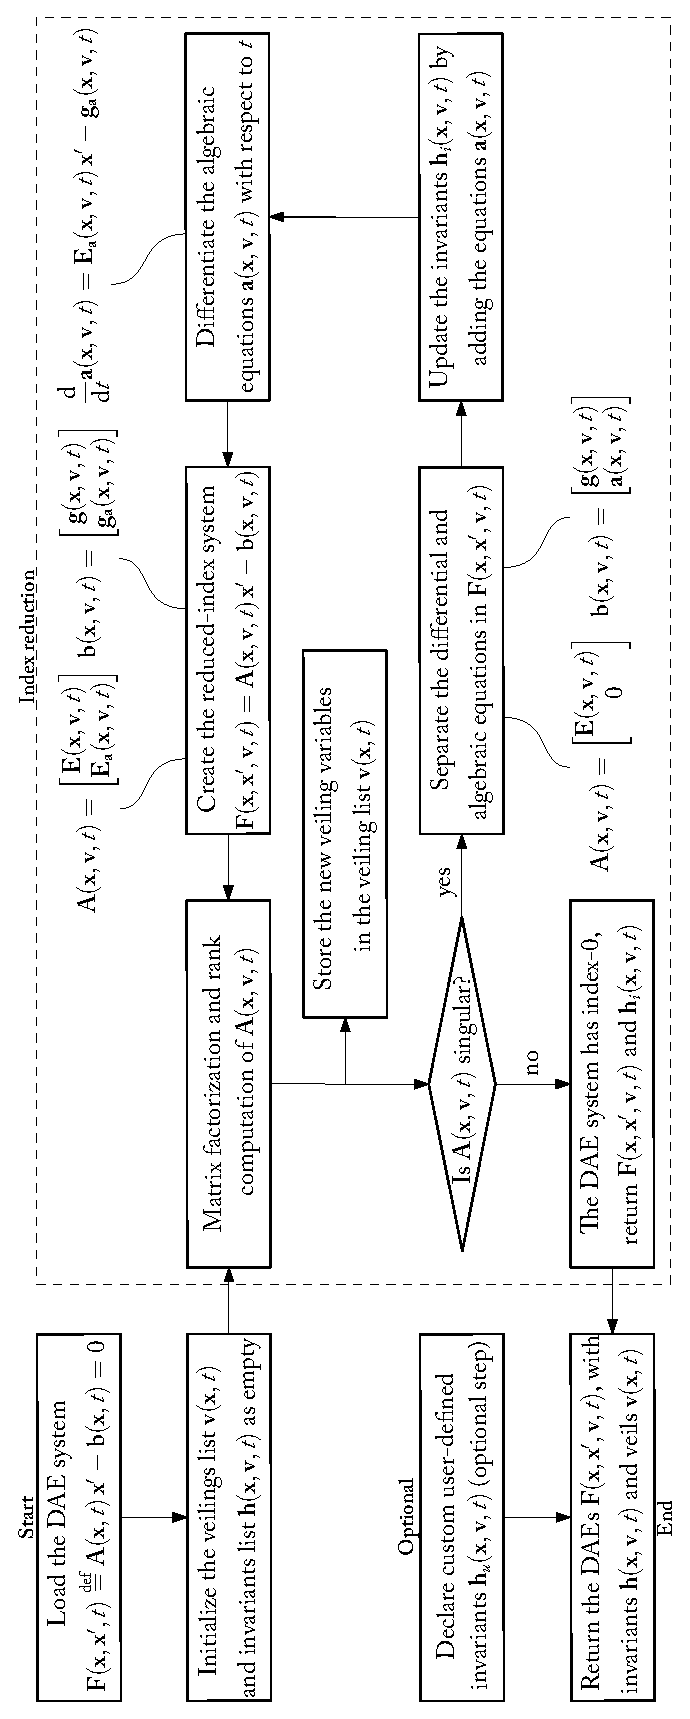
\includegraphics[angle=0, width=0.5\columnwidth]{dae_flowchart_veil}
  \caption{Flowchart of the index reduction algorithm with expression swell mitigation.}
  \label{chap4:fig:index_reduction_veil}
\end{figure}

\begin{breakablealgorithm}
  \caption{Index reduction algorithm with expression swell mitigation.}
  \label{chap4:alg:index_reduction_veil}
  \begin{algorithmic}[1]
    \State \textbf{Require:} A \ac{DAE} system of the form $\mFv \eqdef \mAv \, \mxp - \mbv = \m{0}$.
    \Procedure{ReduceIndex}{$\mFv$} \Comment{Index reduction procedure}
      \State $\mhiv \gets \varnothing$ \Comment{The set of invariants}
      \State $\mv \gets \varnothing$ \Comment{The veiling variables vector}
      \State $\mAv, \, \mbv \gets \mathrm{GenerateMatrix}(\mFv, \, \mxp)$ \Comment{The \ac{DAE} system matrix}
      \State $m \gets \mathrm{Size}(\mx)$\Comment{The size of $\mx$}
      \While{$\mAv$ is singular}
        \State $\displaystyle\triangleright$ Differential and algebraic equations separation (Section~\ref{chap4:sec:separation})
        \State $\mLv, \, \mUv, \, \mP, \, \mQ, \, \m{v}_d(\mx, \m{v}, \, t) \gets \mathrm{MatrixFactorization}(\mAv)$ \Comment{\ac{LU} or \ac{FFLU} decomposition of $\mAv$ with new veiling variables $\m{v}_d(\mx, \m{v}, \, t)$}
        \State $\mv \gets \mv \cup \m{v}_d(\mx, \m{v}, \, t)$ \Comment{Update the veiling variables vector}
        \State $r \gets \mathrm{Rank}(\mUv)$ \Comment{The rank of $\mUv$ is equal to the rank of $\mAv$}
        \State $\mI_1 \gets \mathrm{IdentityMatrix}(r, \, r)$ \Comment{The upper identity matrix}
        \State $\mI_2 \gets \mathrm{IdentityMatrix}(m-r, \, m-r)$ \Comment{The lower identity matrix}
        \State $\mEv \gets \begin{bmatrix} \mI_1, \, \m{0} \end{bmatrix} \, \mUv \, \mQ^\top$ \Comment{The reordered part of $\mAv$}
        \State $\mgv \gets \begin{bmatrix} \mI_1, \, \m{0} \end{bmatrix} \, \mLv^{-1} \, \mP \, \mbv$ \Comment{The differential part of $\mbv$}
        \State $\mav \gets \begin{bmatrix} \m{0}, \, \mI_2 \end{bmatrix} \, \mLv^{-1} \, \mP \, \mbv$ \Comment{The algebraic part of $\mbv$}
        \State $\displaystyle\triangleright$ Algebraic equations differentiation (Section~\ref{chap4:sec:differentiation})
        \State $\jac{\m{v}}{\mx}(\mx, \m{v}, \, t) \gets \mathrm{Jacobian}(\mv, \, \mx)$ \Comment{The Jacobian of $\mav$ with respect to $\mx$}
        \State $\mav \gets \mathrm{Diff}(\mav, \, t)$ \Comment{Differentiate the equations $\mav$}
        \State $\mav \gets \mathrm{Substitute}(\jac{\m{v}}{\mx}(\mx, \m{v}, \, t), \mav)$ \Comment{Remove the $\mv$ derivatives from $\mav$}
        \State $\mAdv, \, \mgdv \gets \mathrm{GenerateMatrix}(\mav, \, \mxp)$ \Comment{Differentiate the equations $\mav$}
        \State $\mAv \gets \begin{bmatrix} \mEv \\ \mAdv \end{bmatrix}$ and $\mbv \gets \begin{bmatrix} \mgv \\ \mgdv \end{bmatrix}$
        \Comment{The new matrix $\mAv$ and vector $\mbv$}
        \State $\mhiv \gets \mhiv \cup \mav$ \Comment{Add the algebraic equations to the set of invariants}
      \EndWhile \\
      \Return $\mAv, \, \mbv, \, \mhiv, \, \mv$ \Comment{The \acp{DAE} reduced to an \ac{ODE} system with invariants}
    \EndProcedure
  \end{algorithmic}
\end{breakablealgorithm}

% % % % % % % % % % % % % % % % % % % % % % % % % % % % % % % % % % % % % % % %

\section{Index Reduction and Numerical Integration Scheme}
\label{chap4:sec:indigo}

After this fairly long discussion on the actual implementation aspects of the index reduction algorithm, we can now present the \Indigo{} index reduction and integration toolbox~\cite{indigo}. This toolbox consists of two main components: a \Maple{} package to carry out symbolic index reduction of \ac{DAE} systems, and a \Matlab{} toolbox to perform numerical integration of the reduced-index system. \Indigo{} is designed to be used in conjunction with the \LEM{} package, to limit the expression swell, and the \LAST{} package, to conveniently factorize matrices. In the following paragraphs, we briefly discuss the usage of the \Indigo{} package.

\subsection{Index Reduction}

The index reduction algorithm implemented in the \Indigo{} \Maple{} package is the one presented in Section~\ref{chap4:sec:algorithm}. To reduce the index of a \ac{DAE} system in the \Maple{} environment we need to first create an \Indigo{} object instance.
%
\begin{verbatim}
> Indigo_obj := Object(Indigo);
> Indigo_obj:-InitLAST();
\end{verbatim}
%
Then, the system of \acp{DAE} \texttt{eqns} with coordinates \texttt{vars} is loaded.
%
\begin{verbatim}
> Indigo_obj:-LoadEquations('Generic', eqns, vars);
\end{verbatim}
%
The \texttt{Generic} symbol is used to specify the type of the system. Notice that in this example, we assume that the equations of the system are already available in the \Maple{} session. The automatic index reduction process can be performed by calling the \texttt{ReduceIndex} method, which iterates the separation and differentiation steps until an index-$0$ \ac{DAE} system is obtained.
%
\begin{verbatim}
> Indigo_obj:-ReduceIndex();
\end{verbatim}
%
Intermediate results of the process are stored internally in the \Indigo{} object and are available on demand. Once the index reduction process is completed, the user can generate the \texttt{SliderCrank} \Matlab{} class file to perform numerical integration of the reduced-index system.
%
\begin{verbatim}
> Indigo_obj:-GenerateMatlabCode(name, type, data=pars);
\end{verbatim}
%
A file \texttt{name.m} is generated in the current directory. As it is explained in the next section, The string parameter \texttt{type} can be either \texttt{Implicit}, \texttt{SemiExplicit} or \texttt{Explicit} depending on the desired numerical integration scheme. The optional parameter \texttt{data} introduces default internal object data.

\subsection{Numerical Integration Scheme}

The \Indigo{} \Matlab{} toolbox is an object-oriented library that allows the user to exploit the automatically generated code of the reduced-index system. It is capable of integrating systems of \acp{ODE} and \acp{DAE} using a variety of \ac{RK} numerical integration schemes. In particular, the system of equations which is integrated is composed of the following elements.
%
\begin{itemize}
  \setlength{\itemsep}{0pt}
    \item A differential part, which can be expressed by one of the following classes:
    %
    \begin{equation*}
        \begin{array}{ccl}
            \m{F}(\mx, \mx^\prime, \m{v}, t) = \m{0} & \hspace{0.5cm} &
            \text{\texttt{Implicit} system class,} \\[0.5mm]
            \m{A}(\mx, \m{v}, t) \, \mx^\prime = \m{b}(\mx, \m{v}, t) & \hspace{0.5cm} &
            \text{\texttt{SemiExplicit} system class,} \\[0.5mm]
            \mx^\prime = \m{f}(\mx, \m{v}, t) & \hspace{0.5cm} &
            \text{\texttt{Explicit} system class.}
        \end{array}
    \end{equation*}
    %
    \item The invariants, composed of the hidden constraints obtained from the index reduction process $\mhiv$, and optional user-defined invariants $\mhuv$, namely
    %
    \begin{equation}
      \label{chap4:eq:inv_part}
      \m{h}(\mx, \m{v}, t) = \begin{bmatrix}
          \mhiv \\[0.5mm]
          \mhuv
      \end{bmatrix} = \m{0} \, \text{.}
    \end{equation}
    %
    \item The veils, which are the set of the expression hierarchical representation variables used in \LEM{} to limit the expression swell
    %
    \begin{equation*}
        \m{v}(\mx, t) = \begin{bmatrix}
            v_{1}(\mx, t) \\[0.5mm]
            v_{2}(v_{1}, \mx, t) \\
            \vdots \\
            v_{n}(v_{1}, \dots, v_{n-1}, \mx, t)
        \end{bmatrix} \, \text{.}
    \end{equation*}
\end{itemize}

To respect the invariants during the integration the \emph{standard projection} method is applied~\cite{hairer2000symmetric}. This method consists of projecting the solution $\mx$ of the numerically integrated reduced-index system onto the invariants manifold $\m{h}(\mx, \m{v}, t) = \m{0}$, which is equivalent to the following constrained minimization
%
\begin{equation*}
  \underset{\widetilde{\mx}}{\textrm{minimize}} \quad \dfrac{1}{2}\left(\mx - \widetilde{\mx}\right)^2
    \quad \textrm{subject to} \quad
    \m{h}(\mx, \m{v}, t) = \m{0}.
\end{equation*}

To integrate the system generated through the \Matlab{} package or a custom system \texttt{sys}, the user must first instantiate a \Indigo{} \ac{RK} solver.
%
\begin{verbatim}
>>> solver = IndigoSolver('solver_name');
>>> solver.set_system(sys);
\end{verbatim}
%
Once the solver is instantiated, it is only necessary to specify the \acp{IC} and the integration time vector.
%
\begin{verbatim}
>>> [x, t, v, h] = solver.solve(t_ini:d_t:t_end, ics);
\end{verbatim}
%
The solver returns the solution of the system in the form of multiple outputs: \texttt{x} contains the integrated solution, \texttt{x\_dot} the states' time derivative, \texttt{t} the time vector, \texttt{v} the veiling variables, and finally \texttt{h} the values of the invariants over the specified time mesh \texttt{t\_ini:d\_t:t\_end}.

% % % % % % % % % % % % % % % % % % % % % % % % % % % % % % % % % % % % % % % %

\section{Proofing the Symbolic-Numeric Scheme}
\label{chap4:sec:example}

In this section, we showcase an example of a high-index \ac{DAE} system: an index-3 problem with an analytical solution, which describes the motion of a particle on a 3D torus surface~\cite{campbell1995constraint}. This example is employed to validate the numerical stability of the reduced-index system, as well as the good conditioning of both the symbolic matrix factorization and the numerical integration scheme. To ease the understanding of the results, we purposely avoid the use of the veiling variables in this example. However, the veiling variables just add an evaluation layer to the expressions, and they do not affect the numerical properties of the integrator.

\subsection{Expression Complexity of the Reduced-Index Systems}
\label{chap4:sec:daes_complexity}

As a first demonstration of the proposed index reduction algorithm capabilities, we first consider the given example from a purely symbolic perspective. In particular, we consider the computational cost of the expressions generated during the presented procedure, both with \ac{LU} and \ac{FFLU} factorization of the system matrix. The compactness of the expressions generated during the index reduction algorithm is a crucial aspect, as it ensures that limited computational overhead is introduced in the numerical integration of the reduced-index system, as well as in the projection of the solution on the hidden constraints. Specifically, the index reduction algorithm is applied to the \ac{DAE} system and reduced to index-0. For each reduction stage of the example considered, the computational cost is reported in Table~\ref{chap4:tab:torus}. Notably, the results show that the expression complexity is similar for both \ac{LU} and \ac{FFLU} factorization, with a slight increase in the number of multiplications and divisions for the latter.

\begin{table}[htp]
  \caption{Expression complexity encountered throughout the index reduction of the particle motion \ac{DAE} system. \emph{Legend}: $\cf$ = functions, $\ca$ = additions, $\cm$ = multiplications, and $\cd$ = divisions.}
  \label{chap4:tab:torus}
  \centering
  {\footnotesize\begin{tabular}{cccc}
    \multicolumn{4}{c}{\textbf{Particle Motion (LU Factorization)~\cite{campbell1995constraint}}} \\
    \toprule
    \textbf{Original \acp{DAE}} & \multicolumn{3}{c}{$\mF = 47\cf + 30\cm + 23\ca$ \quad $\mh = 0$} \\
    \midrule
    \textbf{Reduction step} & $\mE$ & $\mg$ & $\ma$ \\
    \midrule
    Index-3 \acp{DAE} & $0$ & $39\cf + 36\cm + 13\ca$ & $7\cf + 10\cm + 6\ca$ \\
    Index-2 \acp{DAE} & $0$ & $39\cf + 36\cm + 13\ca$ & $22\cf + 20\cm + 8\ca$ \\
    Index-1 \acp{DAE} & $0$ & $39\cf + 36\cm + 13\ca$ & $68\cf + 72\cm + 33\ca$ \\
    Index-0 \acp{DAE} & $388\cf + 424\cm + 180\ca$ & $79\cf + 77\cm + 26\ca$ & $0$ \\
    \midrule
    \textbf{Reduced \acp{DAE}} & \multicolumn{3}{c}{$\mF = 258\cf + 239\cm + 109\ca$ \quad $\mh = 97\cf + 102\cm + 47\ca$} \\
    \bottomrule \\[0.5em]
    %
    \multicolumn{4}{c}{\textbf{Particle Motion (FFLU Factorization)~\cite{campbell1995constraint}}} \\
    \toprule
    \textbf{Original \acp{DAE}} & \multicolumn{3}{c}{$\mF = 47\cf + 30\cm + 23\ca$ \quad $\mh = 0$} \\
    \midrule
    \textbf{Reduction step} & $\mE$ & $\mg$ & $\ma$ \\
    \midrule
    Index-3 \acp{DAE} & $0$ & $39\cf + 36\cm + 13\ca$ & $7\cf + 10\cm + 6\ca$ \\
    Index-2 \acp{DAE} & $0$ & $39\cf + 36\cm + 13\ca$ & $26\cf + 23\cm + 8\ca$ \\
    Index-1 \acp{DAE} & $0$ & $39\cf + 36\cm + 13\ca$ & $68\cf + 72\cm + 33\ca$ \\
    Index-0 \acp{DAE} & $388\cf + 424\cm + 180\ca$ & $79\cf + 77\cm + 26\ca$ & $0$ \\
    \midrule
    \textbf{Reduced \acp{DAE}} & \multicolumn{3}{c}{$\mF = 258\cf + 239\cm + 109\ca$ \quad $\mh = 97\cf + 105\cm + 47\ca$} \\
    \bottomrule
    \end{tabular}}
\end{table}

\subsection{Numerical Integration of the Reduced-Index System}
\label{chap4:sec:numerical_integration}

The numerical stability and consistency of the reduced-index system are demonstrated by exploiting the analytical solution of the problem in~\cite{campbell1995constraint}. Specifically, the \ac{DAE} system consists of three position variables $[x_{1}, \, x_{2}, \, x_{3}]^\top$, three velocity variables $[u_{1}, \, u_{2}, \, u_{3}]^\top$, and one constraint with Lagrange multiplier $\lambda$. The solution manifold is 4D, and the exact solution is
%
\begin{equation}
  \label{chap4:eq:torus_solution}
  \mx_\text{exact} = \begin{bmatrix}
    x_{1} \\ x_{2} \\ x_{3}
  \end{bmatrix} = \begin{bmatrix}
    (\rho \cos(2\pi - t) + r) \cos(t) \\
    (\rho \cos(2\pi - t) + r) \sin(t) \\
    \rho \sin(2\pi - t)
  \end{bmatrix} \, \text{.}
\end{equation}
%
The initial value problem is defined as follows
%
\begin{equation}
  \label{chap4:eq:torus}
  \mF = \begin{bmatrix}
    x^{\prime}_{1} - u_{1} \\
    x^{\prime}_{2} - u_{2} \\
    x^{\prime}_{3} - u_{3} \\
    u^{\prime}_{1} - u_{3}\cos(t) + x_{3}\sin(t) + u_{2} - 2 c x_{1}\lambda \\
    u^{\prime}_{2} - u_{3}\sin(t) - x_{3}\cos(t) - u_{1} - 2 c x_{2}\lambda \\
    u^{\prime}_{3} + x_{3} - 2x_{3}\lambda \\
    x_{1}^2 + x_{2}^2 + x_{3}^2 - 2r(x_{1}^2 + x_{2}^2)^{1/2} + r^2 - \rho^2
  \end{bmatrix} \, \text{,}
\end{equation}
%
with $c = 1 - {r} / {(x_{1}^2 + x_{2}^2)^{1/2}}$, states $\mx = [x_{1}, \, x_{2}, \, x_{3}, \, u_{1}, \, u_{2}, \, u_{3}, \, \lambda]^{\top}$, \acp{IC} $\mx_{0} = [15, \, 0, \, 0, \, 0, \, 15, \, -5, \, \lambda]^{\top}$, and parameters $\rho = 5$ and $r = 10$.

The numerical integration of the reduced-index system is performed through Implicit Euler, RadauIIA3, and RadauIIA5 \ac{RK} methods. To respect the invariants during the integration the \emph{standard projection} method is applied~\cite{hairer2000symmetric}. This method consists of projecting the solution $\mx$ of the numerically integrated system onto the invariants on the hidden constraints $\mh = \m{0}$, which is equivalent to the constrained minimization
%
\begin{equation*}
  \underset{\tilde{\mx}}{\textrm{minimize}} \quad \dfrac{1}{2}\left(\mx - \tilde{\mx}\right)^2
    \quad \textrm{subject to} \quad
    \mh = \m{0} \, \text{.}
\end{equation*}
%
To verify that the projection is performed correctly and does not affect the order of the \ac{RK} method, numerical integration is performed in the interval $t \in [0, \, 2\pi]$ seconds with different integration time steps $\Delta t$. The error of the numerical integration $\varepsilon = \| \, \mx - \mx_\text{exact} \, \|_{\infty}$ is reported in \figurename~\ref{chap4:fig:torus_order}. As it can be seen, the implemented projection preserves the order of the method for all the integration time steps. It is important to highlight that to obtain such results the absolute error tolerances of the integrator and the projection are both set to $\varepsilon = 10^{-10}$. The same tolerances are used in the numerical integration of the reduced-index system in the interval $t \in [0, \, 400\pi]$ seconds with step $\Delta t = 0.025$ seconds. The results are reported in \figurename~\ref{chap4:fig:torus_integration}, where Implicit Euler, RadauIIA3, and RadauIIA5 \ac{RK} methods are employed, and the projection on the hidden constraints $\mh$ is performed. The effect of the projection is highlighted on the bottom left plot.

\begin{figure}[htp]
  \centering
  \includetikz{figures/chapter_3/torus_order.tex}
  \includetikz{figures/chapter_3/torus_hidden.tex}
  \caption{Numerical integration error $\varepsilon = \| \, \mx - \mx_\text{exact} \, \|_{\infty}$ of the \acp{DAE}~\eqref{chap4:eq:torus} over different integration time steps $\Delta t$, along with the computed order of the method (left). The projection on the hidden constraints is performed and the invariants violation $\| \, \mh \, \|_{\infty}$ is reported (right). Notice that the implemented projection preserves the order of the method for all the integration time steps. The tests are performed in the interval $t \in [0, \, 2\pi]$ seconds, using Implicit Euler, RadauIIA3, and RadauIIA5 Runge-Kutta methods.}
  \label{chap4:fig:torus_order}
\end{figure}

\begin{figure}[htp]
  \centering
  \includetikz{figures/chapter_3/torus_implicit_euler.tex}
  \includetikz{figures/chapter_3/torus_radauiia3.tex}
  \includetikz{figures/chapter_3/torus_radauiia5.tex}
  \includetikz{figures/chapter_3/torus_radauiia5_noproj.tex}
  \caption{Numerically integrated solution of the \acp{DAE}~\eqref{chap4:eq:torus} in the interval $t \in [0, \, 400\pi]$ seconds, with step $\Delta t = 0.025$ seconds, using Implicit Euler (top left), RadauIIA3 (top right), and RadauIIA5 (bottom left and right) Runge-Kutta methods. The first three plots show the numerical integration of the reduced-index system with projection on the hidden constraints $\mh$ produced by the index reduction algorithm. On the bottom right plot, the numerical integration of the reduced-index system is performed without projection on the manifold $\mh$ and substantial drift is observed.}
  \label{chap4:fig:torus_integration}
\end{figure}

% % % % % % % % % % % % % % % % % % % % % % % % % % % % % % % % % % % % % % % %